\documentclass[aip,jcp,preprint,noshowkeys,superscriptaddress]{revtex4-1}
\usepackage{graphicx,dcolumn,bm,xcolor,microtype,multirow,amscd,amsmath,amssymb,amsfonts,physics,wrapfig,txfonts,setspace}
\usepackage{siunitx}[=v2]
\usepackage[version=4]{mhchem}
\usepackage{natbib}
\bibliographystyle{achemso}

\maxdeadcycles=200

\newcommand{\fk}[1]{\textcolor{orange}{#1}}

\newcommand{\ie}{\textit{i.e.}}
\newcommand{\eg}{\textit{e.g.}}
\newcommand{\alert}[1]{\textcolor{black}{#1}}
\usepackage[normalem]{ulem}
\newcommand{\titou}[1]{\textcolor{red}{#1}}
\newcommand{\trashPFL}[1]{\textcolor{red}{\sout{#1}}}
\newcommand{\PFL}[1]{\titou{(\underline{\bf PFL}: #1)}}
\newcommand{\toto}[1]{\textcolor{green}{#1}}
\newcommand{\trashAS}[1]{\textcolor{green}{\sout{#1}}}
\newcommand{\AS}[1]{\toto{(\underline{\bf AS}: #1)}}
\newcommand{\ant}[1]{\textcolor{orange}{#1}}
\newcommand{\SupInf}{\textcolor{blue}{Supporting Information}}

\newcommand{\mc}{\multicolumn}
\newcommand{\fnm}{\footnotemark}
\newcommand{\fnt}{\footnotetext}
\newcommand{\tabc}[1]{\multicolumn{1}{c}{#1}}
\newcommand{\QP}{\textsc{quantum package}}

\newcommand{\Ndet}{N_\text{det}}

\newcommand{\EHF}{E_\text{HF}}
\newcommand{\EDOCI}{E_\text{DOCI}}
\newcommand{\EFCI}{E_\text{FCI}}

\renewcommand{\thesection}{S\arabic{section}}
\renewcommand{\thetable}{S\arabic{table}}
\renewcommand{\thefigure}{S\arabic{figure}}
\renewcommand{\theequation}{S\arabic{equation}}

\usepackage[
	colorlinks=true,
    citecolor=blue,
    breaklinks=true
	]{hyperref}
\urlstyle{same}

\begin{document}

\newcommand{\LCPQ}{Laboratoire de Chimie et Physique Quantiques (UMR 5626), Universit\'e de Toulouse, CNRS, UPS, France}

\title{Supporting Information for ``Seniority and Hierarchy Configuration Interaction for Radicals and Excited States''}

\author{F\'abris Kossoski}
\email{fkossoski@irsamc.ups-tlse.fr}
\affiliation{\LCPQ}
\author{Pierre-Fran\c{c}ois Loos}
\email{loos@irsamc.ups-tlse.fr}
\affiliation{\LCPQ}

% Abstract
\begin{abstract}
%Here comes the abstract.
%\bigskip
%\begin{center}
%        \boxed{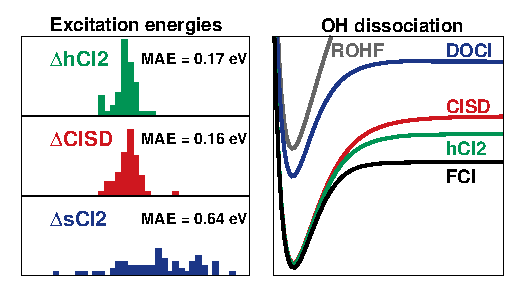
\includegraphics[width=0.4\linewidth]{TOC}}
%\end{center}
%\bigskip
\end{abstract}

% Title
\maketitle

%%%%%%%%%%%%%%%%%%%%%%%%%%%%%%%%%%%%%%%%%%%%%%%%%%
%\section{Statistical measures}
%\label{sec:stat}
%%%%%%%%%%%%%%%%%%%%%%%%%%%%%%%%%%%%%%%%%%%%%%%%%%

\fk{
Given two sets of $N$ paired variables $x_i$ and $y_i$
(in our case, the approximate and reference excitation energies),
the corresponding mean signed error (MSE), mean absolute error (MAE), root-mean-square error (RMSE), and standard deviation of the errors (SDE) are defined as:
}

\begin{equation}
	\fk{\text{MSE} = \frac{1}{N} \sum_{i=1}^{N} (x_i - y_i),}
\end{equation}

\begin{equation}
	\fk{\text{MAE} = \frac{1}{N} \sum_{i=1}^{N} |x_i - y_i|,}
\end{equation}

\begin{equation}
	\fk{\text{RMSE} = \sqrt{ \frac{1}{N} \sum_{i=1}^{N} (x_i - y_i)^2 },}
\end{equation}

\begin{equation}
	\fk{\text{SDE} = \sqrt{ \frac{1}{N} \sum_{i=1}^{N} (x_i - \mu)^2 },}
\end{equation}

\fk{where}
\begin{equation}
	\fk{\mu = \frac{1}{N} \sum_{i=1}^{N} x_i.}
\end{equation}

%%%%%%%%%%%%%%%%%%%%%%%%%%%%%%%%%%%%%%%%%%%%%%%%%%
%\section{Equilibrium geometry of ethylene}
%\label{sec:ethylene}
%%%%%%%%%%%%%%%%%%%%%%%%%%%%%%%%%%%%%%%%%%%%%%%%%%

Equilibrium geometry of ethylene, in atomic units, obtained from Ref. \onlinecite{Loos_2018}:
\begin{singlespace}
\begin{verbatim}
C    0.00000000       1.26026583        0.00000000
C    0.00000000      -1.26026583        0.00000000
H    0.00000000       2.32345976        1.74287672
H    0.00000000      -2.32345976        1.74287672
H    0.00000000       2.32345976       -1.74287672
H    0.00000000      -2.32345976       -1.74287672
\end{verbatim}
\end{singlespace}

Equilibrium geometry of vinyl, in atomic units, obtained from Ref. \onlinecite{Loos_2020}:
\begin{singlespace}
\begin{verbatim}
C    0.00000000       1.16769663       -0.04303146
C    0.00000000      -1.29945364        0.15810072
H    0.00000000       2.38429609        1.59801822
H    0.00000000       2.08759130       -1.87998309
H    0.00000000      -2.90307925       -1.08814513
\end{verbatim}
\end{singlespace}

\clearpage

%%%%%%%%%%%%%%%%%%%%%%%%%%%%%%%%%%%%%%%%%%%%%%%%%%
%\section{\ce{Computational details}}
%\label{sec:comp_details}
%%%%%%%%%%%%%%%%%%%%%%%%%%%%%%%%%%%%%%%%%%%%%%%%%%

\fk{
By fitting the computed potential energy curves with a Morse potential $V(r) = D [1 - e^{-a(r-r_e)}]^2 + C $,
we obtained equilibrium geometries $r_e$, force constants $2Da^2$, and harmonic vibrational frequencies $\left( Da^2/2\pi^2\mu \right)^{1/2}$,
where $\mu$ is the reduced mass.
Since the fitting is restricted to the equilibrium region, employing more elaborate functions would be inconsequential, such that the adopted Morse potential is well justified.
The fitting was performed with the Marquardt-Levenberg algorithm implemented in Gnuplot.
}
The following intervals have been considered for the fitting:
\begin{itemize}
\item \ce{HF}: \SI{0.8}{\angstrom} to \SI{1.3}{\angstrom}
\item \ce{F2}: \SI{1.25}{\angstrom} to \SI{1.65}{\angstrom}
\item ethylene: \SI{2.2}{\bohr} to \SI{2.9}{\bohr}
\item \ce{N2}: \SI{0.95}{\angstrom} to \SI{1.3}{\angstrom}
\item \ce{H4}: \SI{1.45}{\bohr} to \SI{1.95}{\bohr}
\item \ce{H8}: \SI{1.6}{\bohr} to \SI{2.05}{\bohr}
\item \ce{OH}: \SI{0.85}{\angstrom} to \SI{1.2}{\angstrom}
\item \ce{CN}: \SI{1.0}{\angstrom} to \SI{1.4}{\angstrom}
\item vinyl: \SI{2.35}{\bohr} to \SI{2.7}{\bohr}
\item \ce{H7}: \SI{1.6}{\bohr} to \SI{2.05}{\bohr}
\end{itemize}

\clearpage

The non-parallelity error and distance error were computed for the following intervals:
\begin{itemize}
\item \ce{HF}: \SI{0.5}{\angstrom} to \SI{6}{\angstrom}
\item \ce{F2}: \SI{0.95}{\angstrom} to \SI{8}{\angstrom}
\item ethylene: \SI{1.5}{\bohr} to \SI{16}{\bohr}
\item \ce{N2}: \SI{0.7}{\angstrom} to \SI{4}{\angstrom}
\item \ce{H4}: \SI{1}{\bohr} to \SI{10}{\bohr}
\item \ce{H8}: \SI{1}{\bohr} to \SI{10}{\bohr}
\item \ce{OH}: \SI{0.6}{\angstrom} to \SI{8}{\angstrom}
\item \ce{CN}: \SI{0.7}{\angstrom} to \SI{4}{\angstrom}
\item vinyl: \SI{1.7}{\bohr} to \SI{9}{\bohr}
\item \ce{H7}: \SI{1}{\bohr} to \SI{10}{\bohr}
\end{itemize}

\clearpage

\begin{table}[ht!]
\caption{\fk{Number of Determinants in Hierarchy-, Excitation, and Seniority-Based CI Routes, as well as in Full CI, for \ce{OH}, \ce{CN}, vinyl, and \ce{H7},
with the cc-pVDZ basis set and frozen-core approximation.}}
\label{tab:ndet_open}
{\color{orange}
\begin{ruledtabular}
\begin{tabular}{lrrrr}
method &     \ce{OH} &         \ce{CN} &                 vinyl &     \ce{H7} \\
\hline
RHF    &           1 &               1 &                     1 &           1 \\
\hline
CIS    &         131 &             280 &                   533 &         221 \\
CISD   &       5 871 &          27 559 &               100 983 &      16 403 \\
CISDT  &     110 031 &       1 196 384 &             8 620 123 &     491 695 \\
CISDTQ &   1 035 501 &      27 468 434 &           397 093 838 &   7 015 800 \\
\hline
CIs1   &      58 140 &       8 288 280 &         1 160 068 104 &     209 440 \\
CIs3   &   1 686 060 &     530 449 920 &       143 268 410 844 &   9 948 400 \\
CIs5   &  12 267 540 &   9 233 143 920 &     4 974 952 064 004 & 107 338 000 \\
\hline
hCI1   &         299 &             658 &                 1 268 &         500 \\
hCI1.5 &       3 491 &          11 809 &                35 813 &      11 009 \\
hCI2   &      25 401 &         136 234 &               569 178 &      96 290 \\
hCI2.5 &     162 265 &       1 417 234 &             8 899 178 &     832 850 \\
hCI3   &     732 107 &      10 879 834 &           102 007 753 &   5 530 745 \\
hCI3.5 &   2 706 807 &      71 632 834 &         1 011 139 788 &  23 829 890 \\
hCI4   &   7 774 870 &     384 458 809 &         8 484 940 738 &  92 360 660 \\
\hline
FCI    &  45 070 128 & 446 075 229 600 & 4 672 770 853 882 482 & 342 696 200 \\
\end{tabular}
\end{ruledtabular}
}
\end{table}

\begin{table}[ht!]
\caption{\fk{Number of Determinants in Hierarchy-, Excitation, and Seniority-Based CI Routes, as well as in Full CI, for \ce{H4}, \ce{N2}, \ce{F2}, \ce{HF}, \ce{H8}, and ethylene,
with the cc-pVDZ basis set and frozen-core approximation.}}
\label{tab:ndet_closed}
{\color{orange}
\begin{ruledtabular}
\begin{tabular}{lrrr}
method & \ce{H4} &       \ce{N2} &         \ce{F2} \\
\hline
RHF    &       1 &             1 &               1 \\
\hline
CIS    &      73 &           211 &             267 \\
CISD   &   1 675 &        15 436 &          25 138 \\
CISDT  &  12 691 &       483 036 &       1 048 174 \\
CISDTQ &  36 100 &     7 745 886 &      23 236 165 \\
\hline
CIs0   &     190 &        65 780 &         657 800 \\
CIs2   &   7 030 &     6 972 680 &      88 145 200 \\
CIs4   &  36 100 &   145 110 680 &   2 450 305 000 \\
\hline
hCI1   &     109 &           316 &             400 \\
hCI1.5 &     757 &         2 836 &           3 592 \\
hCI2   &   3 052 &        34 336 &          57 457 \\
hCI2.5 &  17 740 &       311 536 &         531 469 \\
hCI3   &  36 100 &     1 913 836 &       4 209 850 \\
hCI3.5 &  36 100 &    11 489 836 &      28 628 650 \\
hCI4   &  36 100 &    49 045 711 &     153 775 000 \\
\hline
FCI    &  36 100 & 4 327 008 400 & 432 700 840 000 \\
\hline
\hline
& & & \\
\hline
\hline
method &    \ce{HF} &       \ce{H8} &           ethylene \\
\hline
RHF    &          1 &             1 &                  1 \\
\hline
CIS    &        113 &           289 &                409 \\
CISD   &      4 341 &        28 585 &             58 855 \\
CISDT  &     68 405 &     1 174 345 &          3 731 535 \\
CISDTQ &    531 595 &    23 805 835 &        124 764 480 \\
\hline
CIs0   &      3 060 &        91 390 &          3 838 380 \\
CIs2   &    174 420 &    13 251 550 &        786 867 900 \\
CIs4   &  1 845 180 &   358 705 750 &     33 086 835 600 \\
\hline
hCI1   &        169 &           433 &                613 \\
hCI1.5 &      1 065 &         5 905 &              8 365 \\
hCI2   &      9 255 &        62 605 &            134 590 \\
hCI2.5 &     55 119 &       879 085 &          1 952 230 \\
hCI3   &    227 109 &     5 659 525 &         17 306 800 \\
hCI3.5 &    856 101 &    40 616 965 &        163 795 120 \\
hCI4   &  2 216 460 &   213 974 380 &      1 112 401 240 \\
\hline
FCI    &  9 363 600 & 8 352 132 100 & 14 733 161 024 400 \\
\end{tabular}
\end{ruledtabular}
}
\end{table}

\clearpage

%%% FIG S1 %%%
\begin{figure*}%[h!]
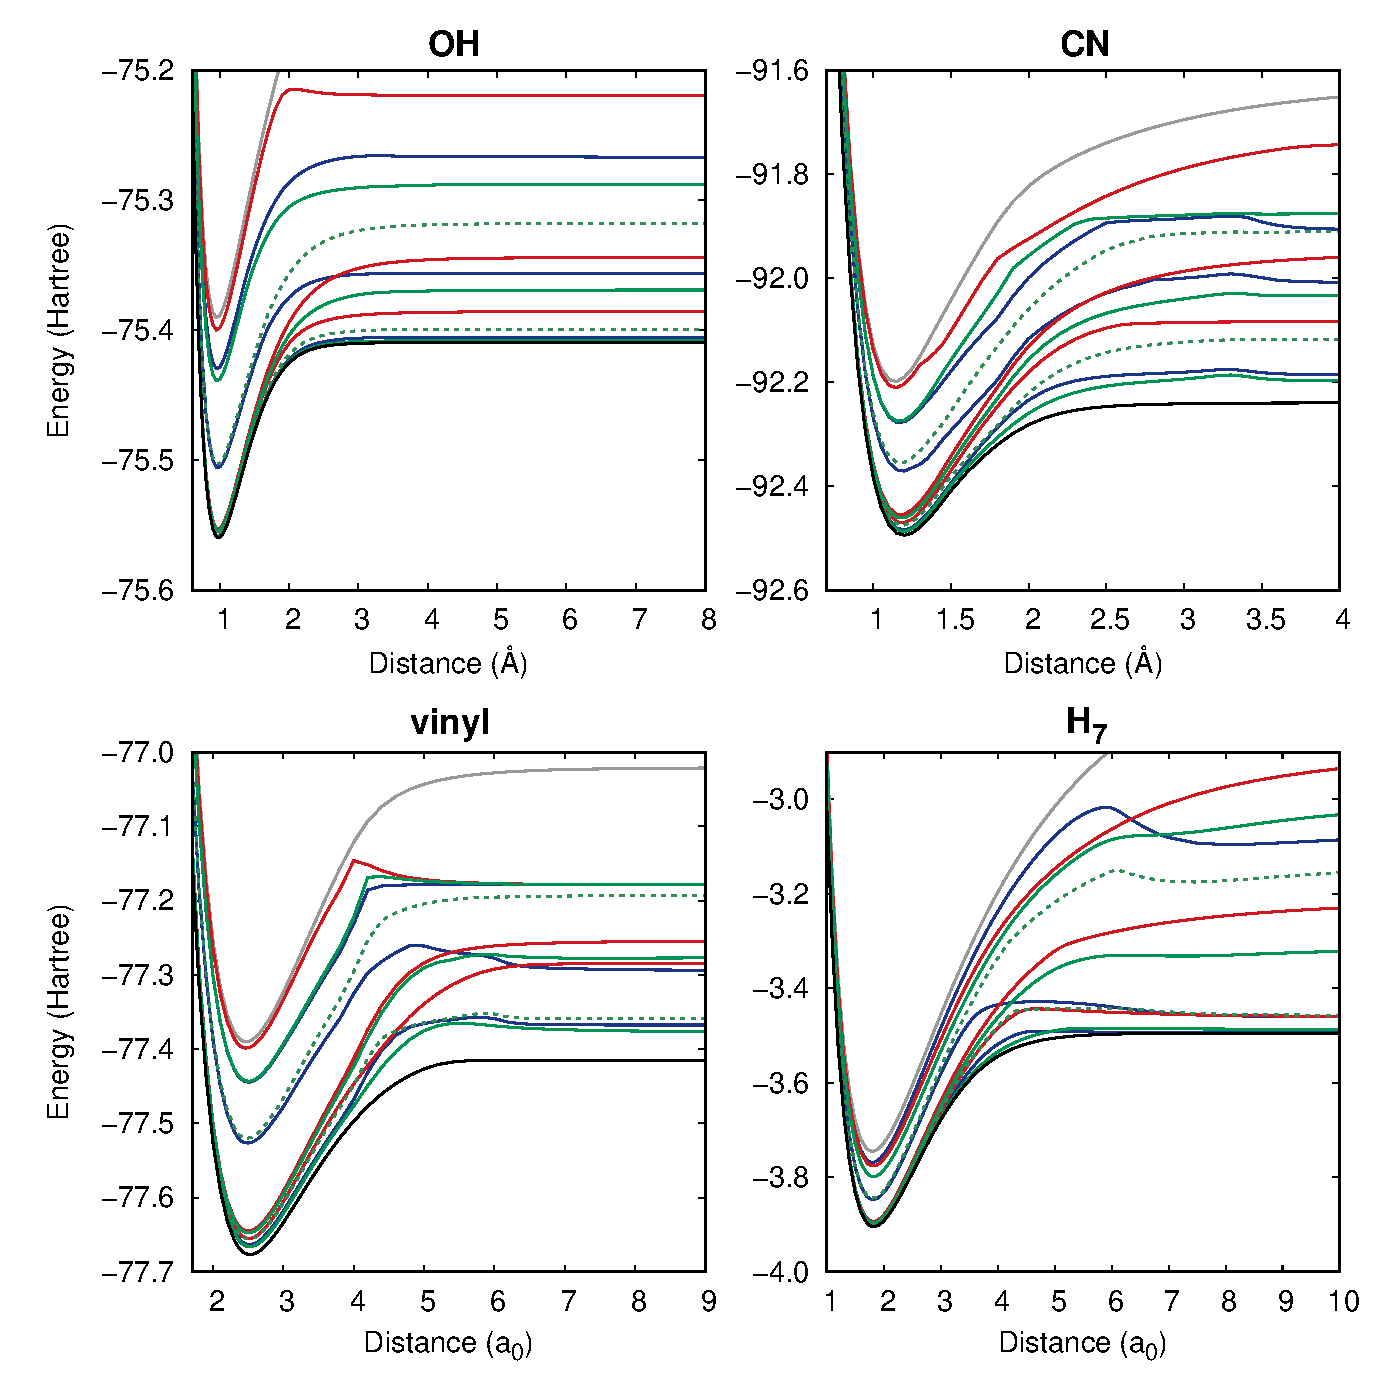
\includegraphics[width=1.0\linewidth]{plot_pes}
\caption{
Potential energy curves for \ce{OH}, \ce{CN}, vinyl, and \ce{H7},
according to restricted open-shell HF (gray), FCI (black), hCI (green) (dashed lines for half-integer $h$), eCI (red), and sCI (blue) models, with the cc-pVDZ basis set and frozen-core approximation.}
\label{fig:plot_pes}
\end{figure*}
%%% %%% %%%

%%% FIG S2 %%%
\begin{figure*}%[h!]
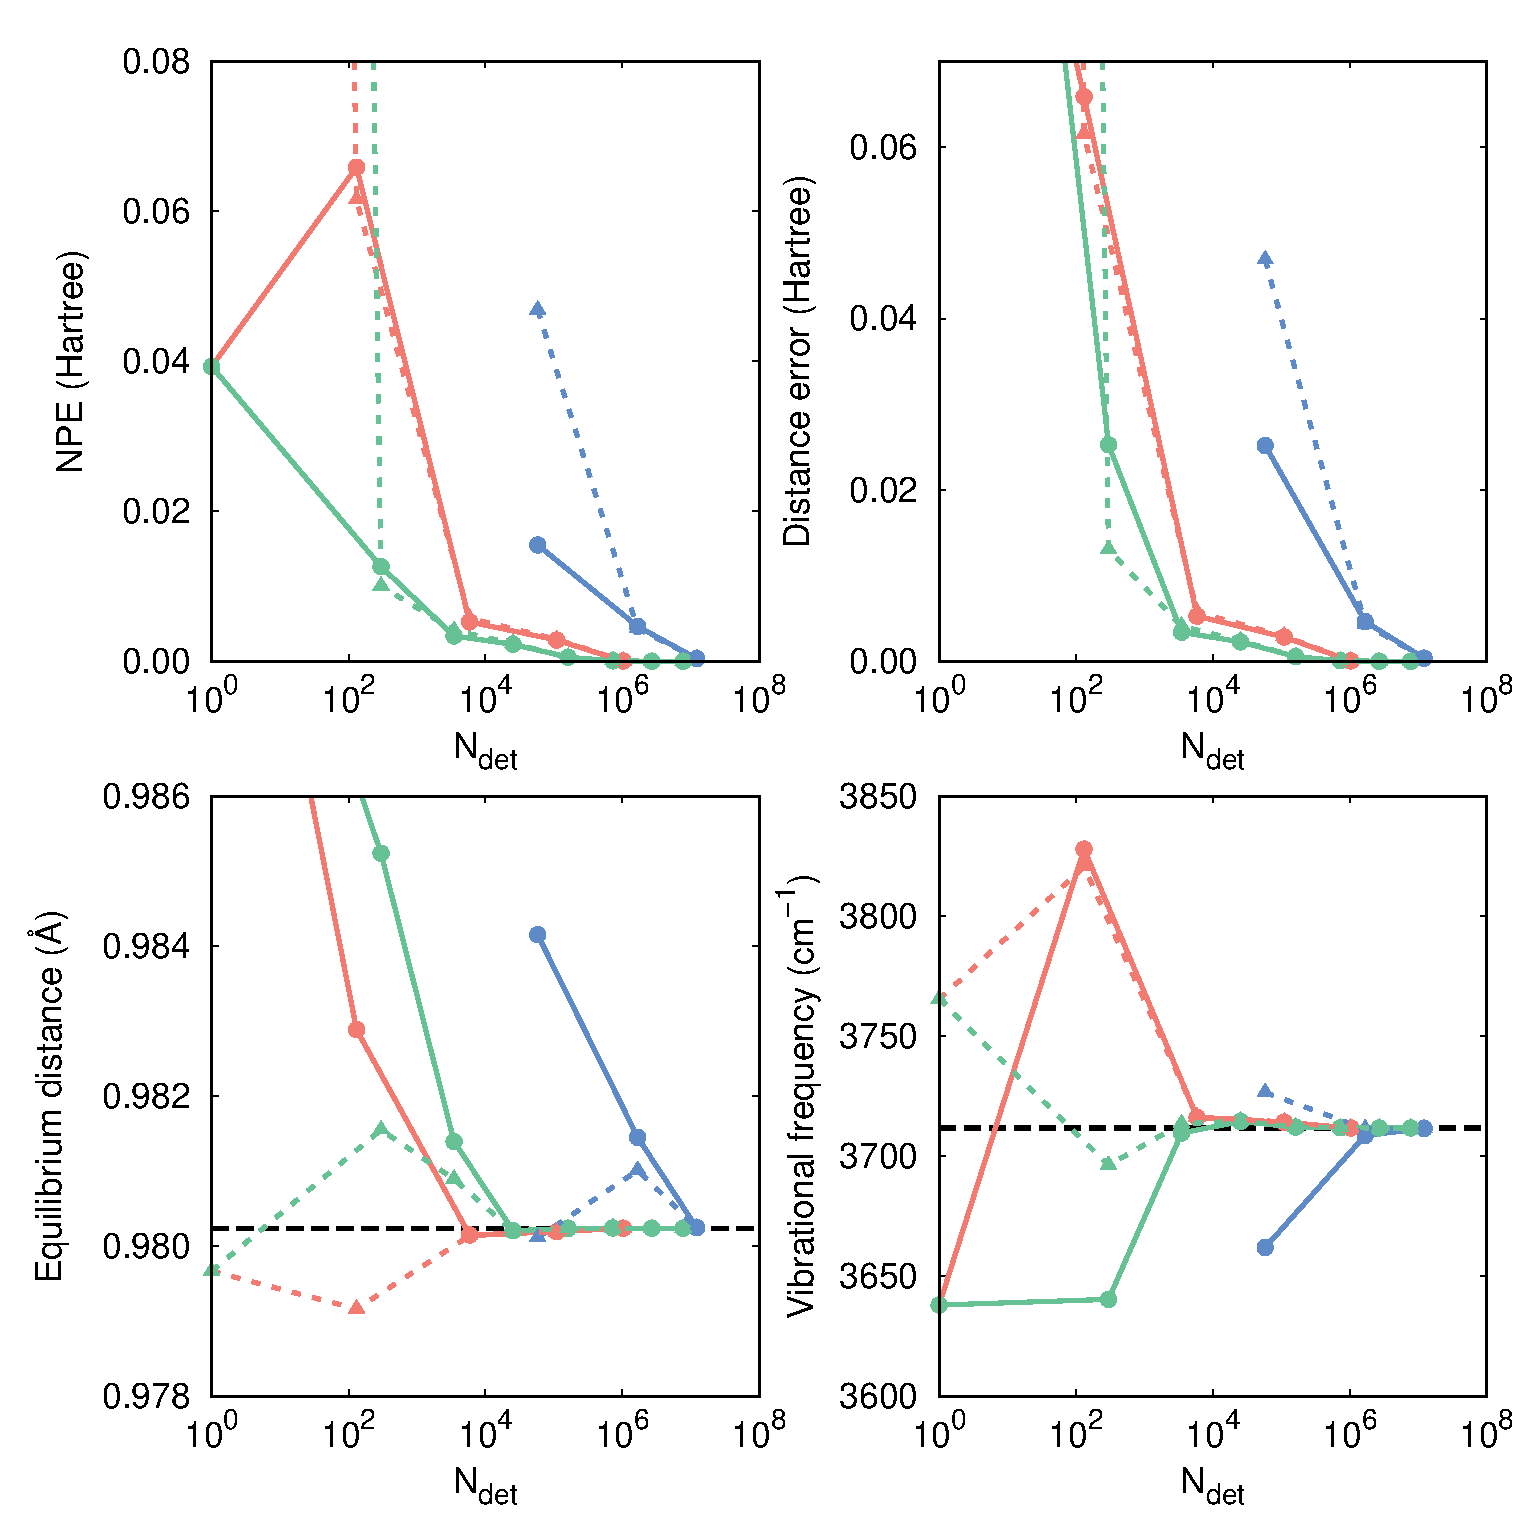
\includegraphics[width=1.0\linewidth]{plot_pt2_rpt2_OH}
\caption{
Non-parallelity error (NPE), distance error, equilibrium distance, and vibrational frequency, for \ce{OH},
as a function of the number of determinants ($\Ndet$), according to hCI (green), eCI (red) and sCI (blue) models,
with the standard (full lines with circles) and renormalized (dashed lines with triangles) EN2 perturbative correction.
The dashed lines represent the FCI results.}
\label{fig:plot_pt2_rpt2_oh}
\end{figure*}
%%% %%% %%%

%%% FIG S3 %%%
\begin{figure*}%[h!]
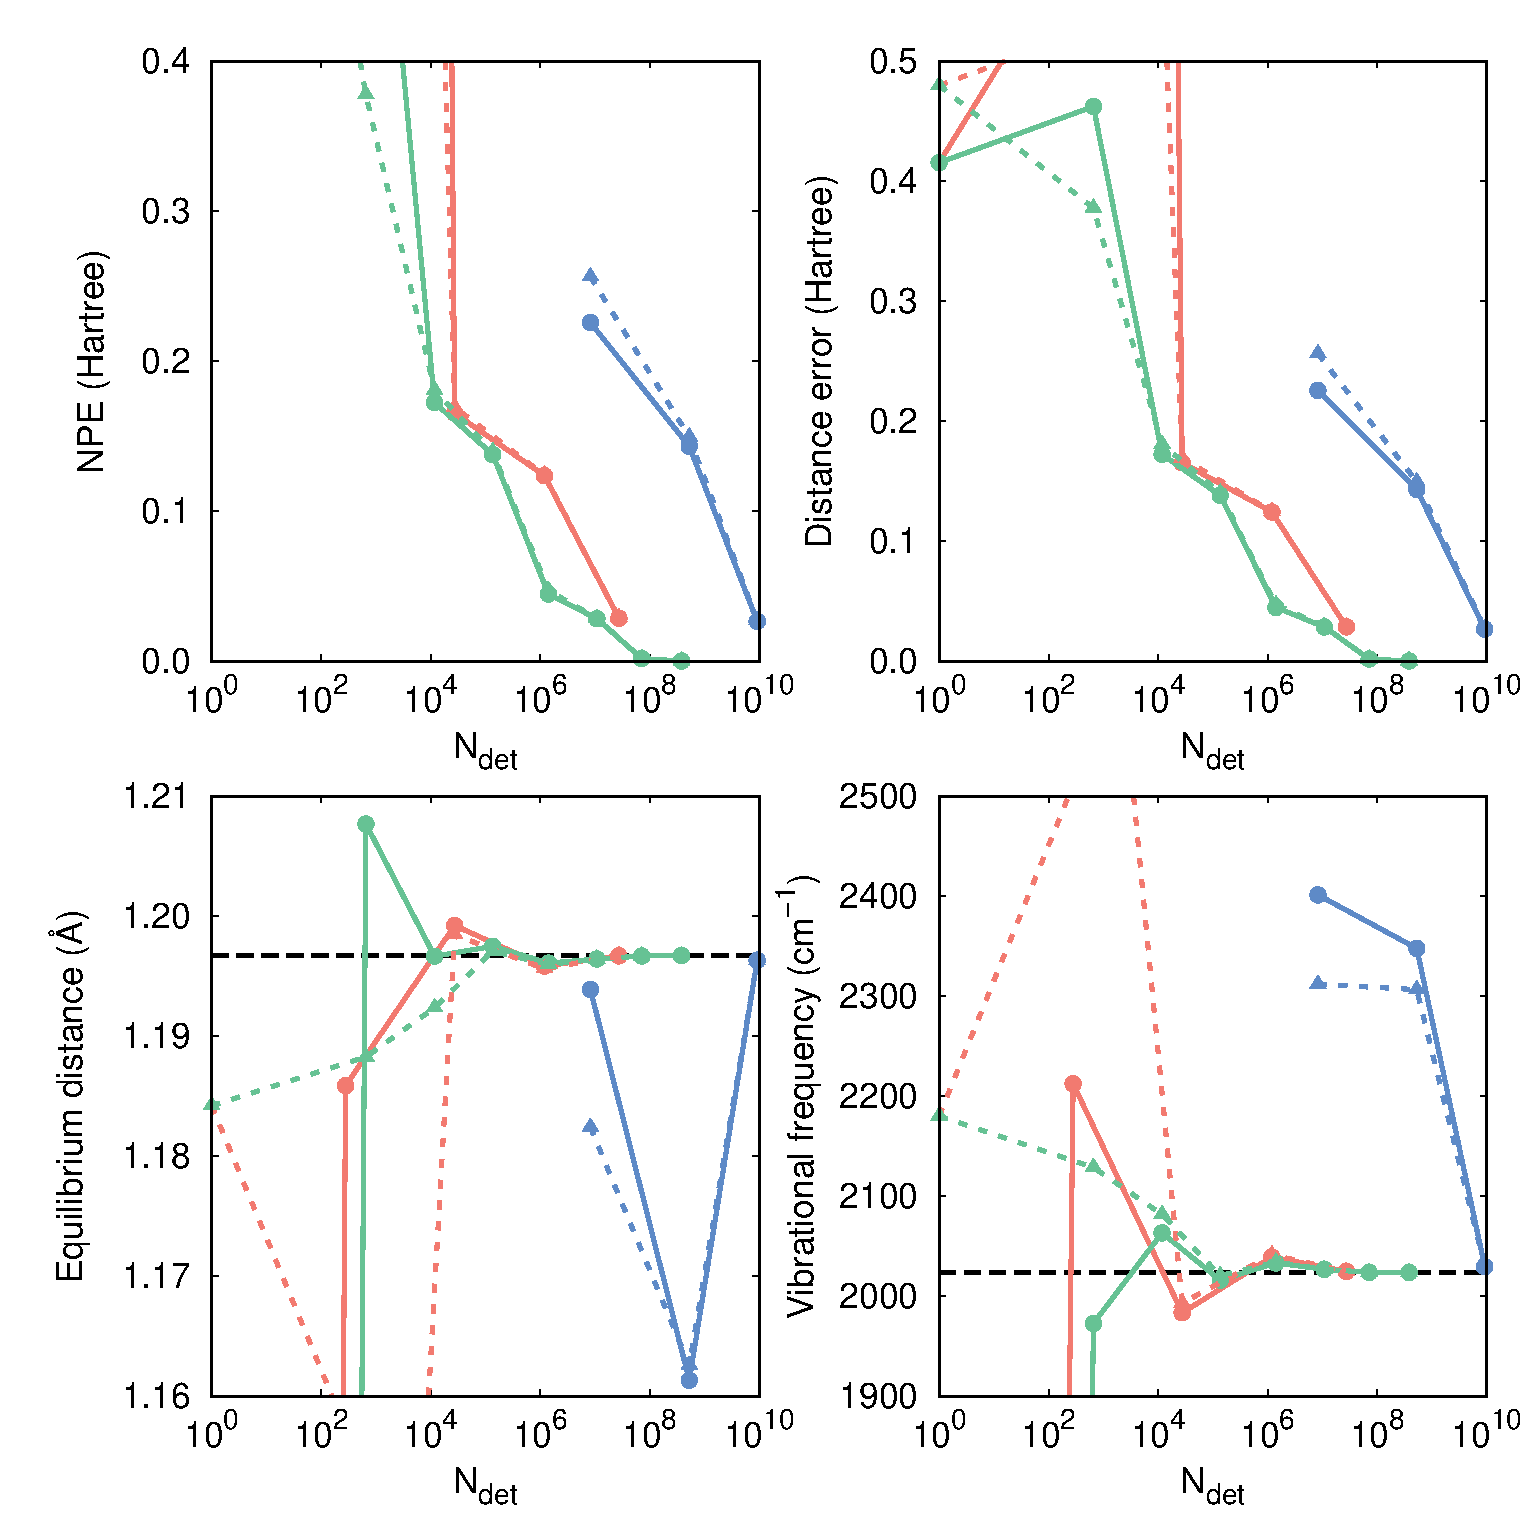
\includegraphics[width=1.0\linewidth]{plot_pt2_rpt2_CN}
\caption{
Non-parallelity error (NPE), distance error, equilibrium distance, and vibrational frequency, for \ce{CN},
as functions of the number of determinants ($\Ndet$), according to hCI (green), eCI (red) and sCI (blue) models,
with the standard (full lines with circles) and renormalized (dashed lines with triangles) EN2 perturbative correction.
The dashed lines represent the FCI results.}
\label{fig:plot_pt2_rpt2_cn}
\end{figure*}
%%% %%% %%%

%%% FIG S4 %%%
\begin{figure*}%[h!]
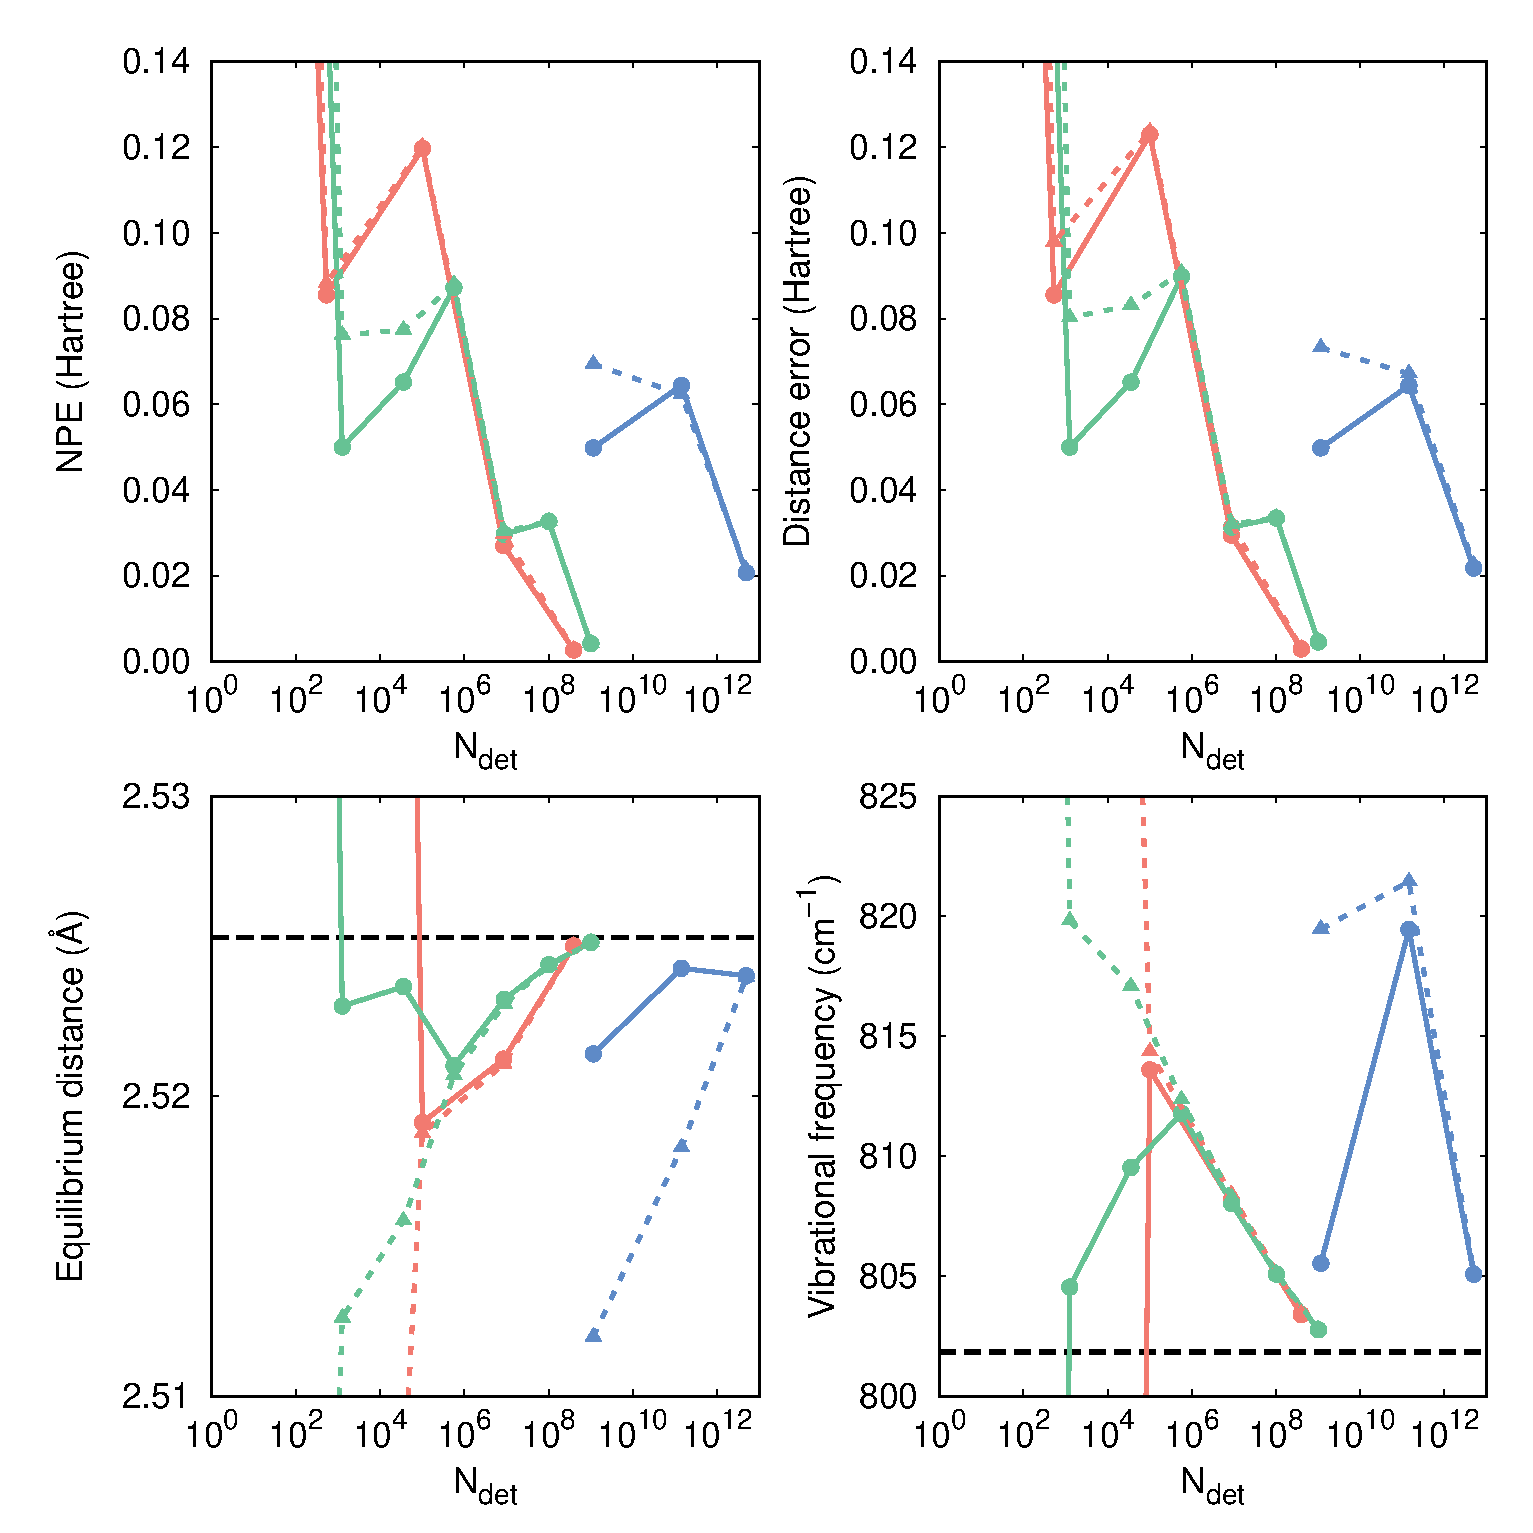
\includegraphics[width=1.0\linewidth]{plot_pt2_rpt2_vinyl}
\caption{
Non-parallelity error (NPE), distance error, equilibrium distance, and vibrational frequency, for vinyl,
as functions of the number of determinants ($\Ndet$), according to hCI (green), eCI (red) and sCI (blue) models,
with the standard (full lines with circles) and renormalized (dashed lines with triangles) EN2 perturbative correction.
The dashed lines represent the FCI results.}
\label{fig:plot_pt2_rpt2_vinyl}
\end{figure*}
%%% %%% %%%

%%% FIG S5 %%%
\begin{figure*}%[h!]
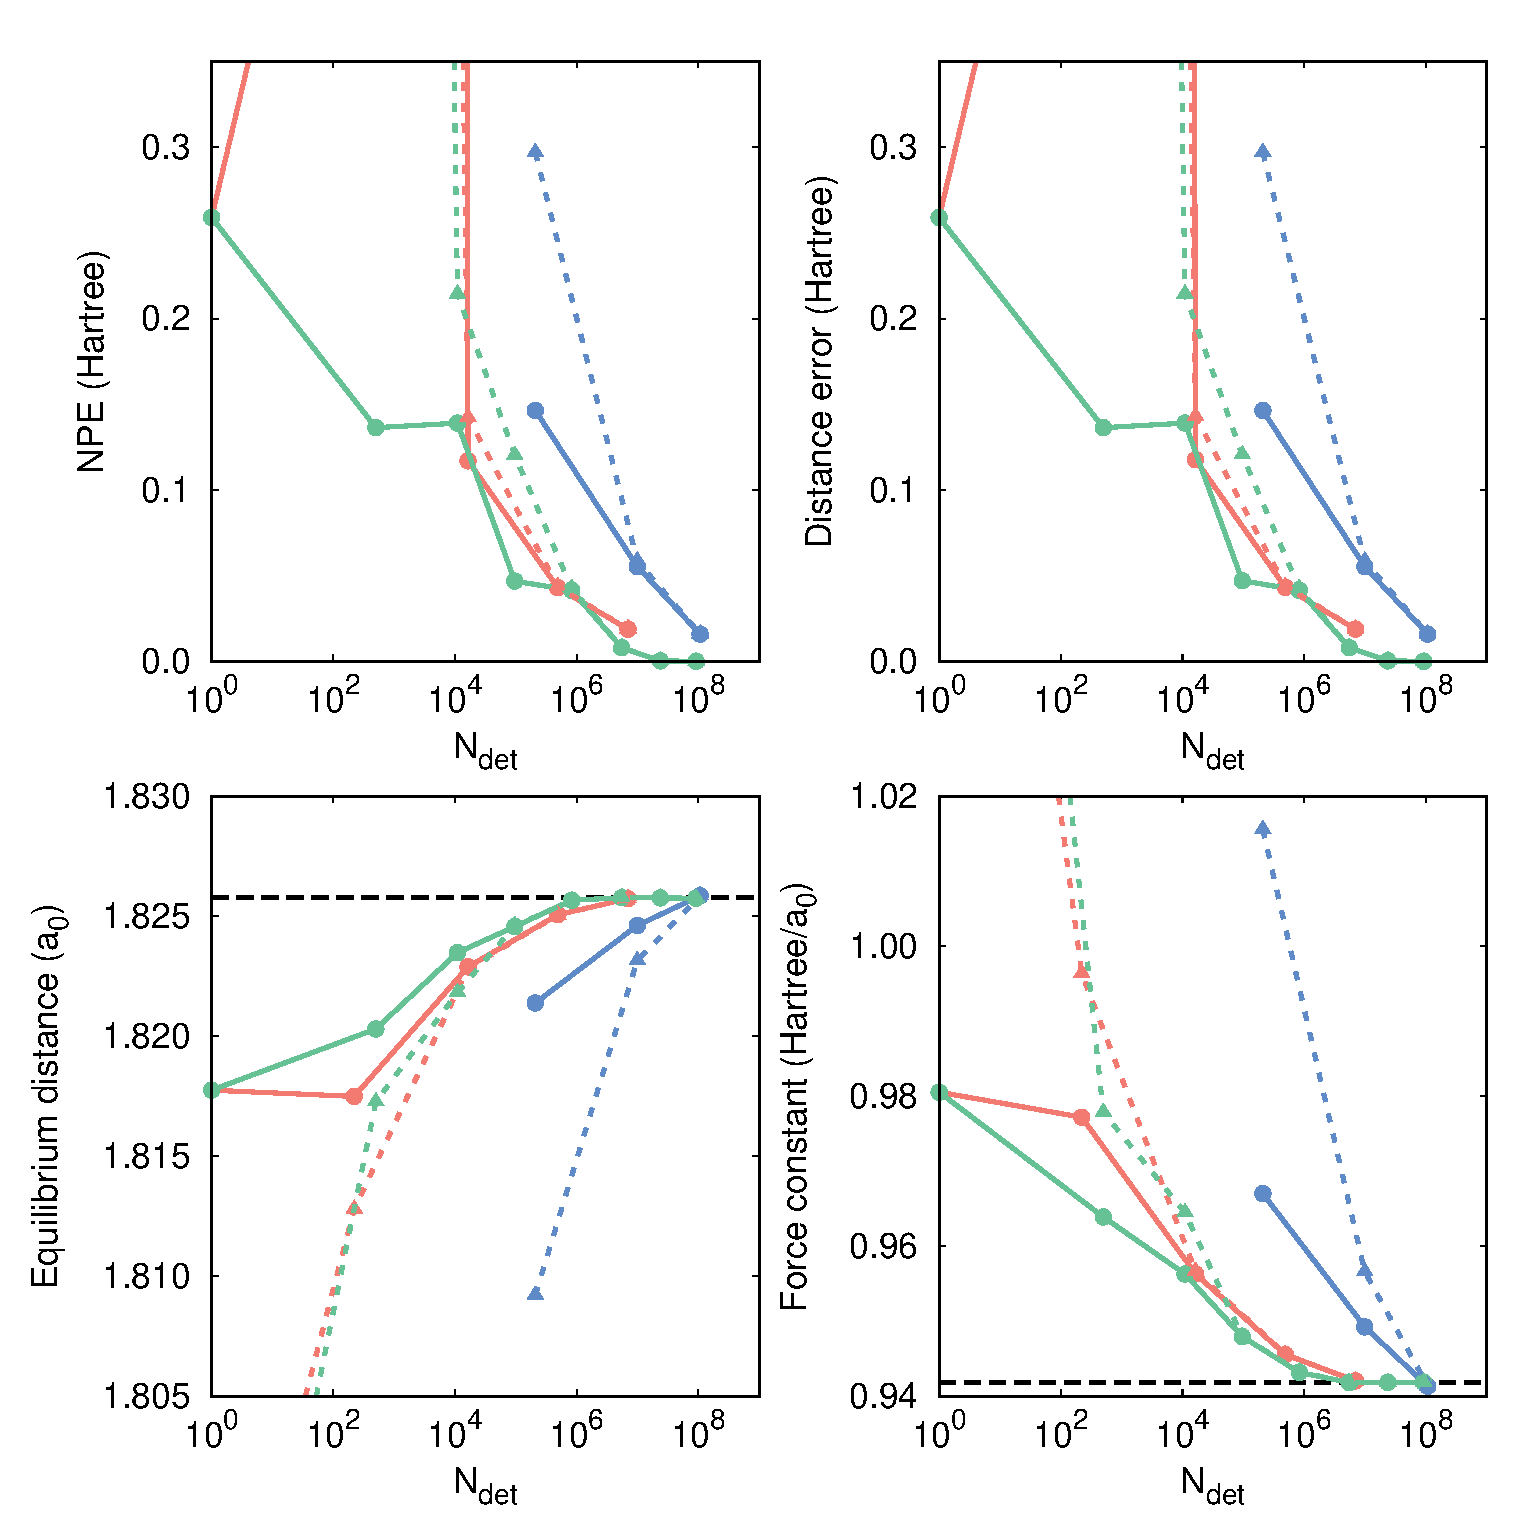
\includegraphics[width=1.0\linewidth]{plot_pt2_rpt2_H7}
\caption{
\label{fig:plot_pt2_rpt2_h7}
Non-parallelity error (NPE), distance error, equilibrium distance, and force constant, for \ce{H7},
as functions of the number of determinants ($\Ndet$), according to hCI (green), eCI (red) and sCI (blue) models,
with the standard (full lines with circles) and renormalized (dashed lines with triangles) EN2 perturbative correction.
The dashed lines represent the FCI results.}
\end{figure*}
%%% %%% %%%

%%% FIG S6 %%%
\begin{figure*}%[h!]
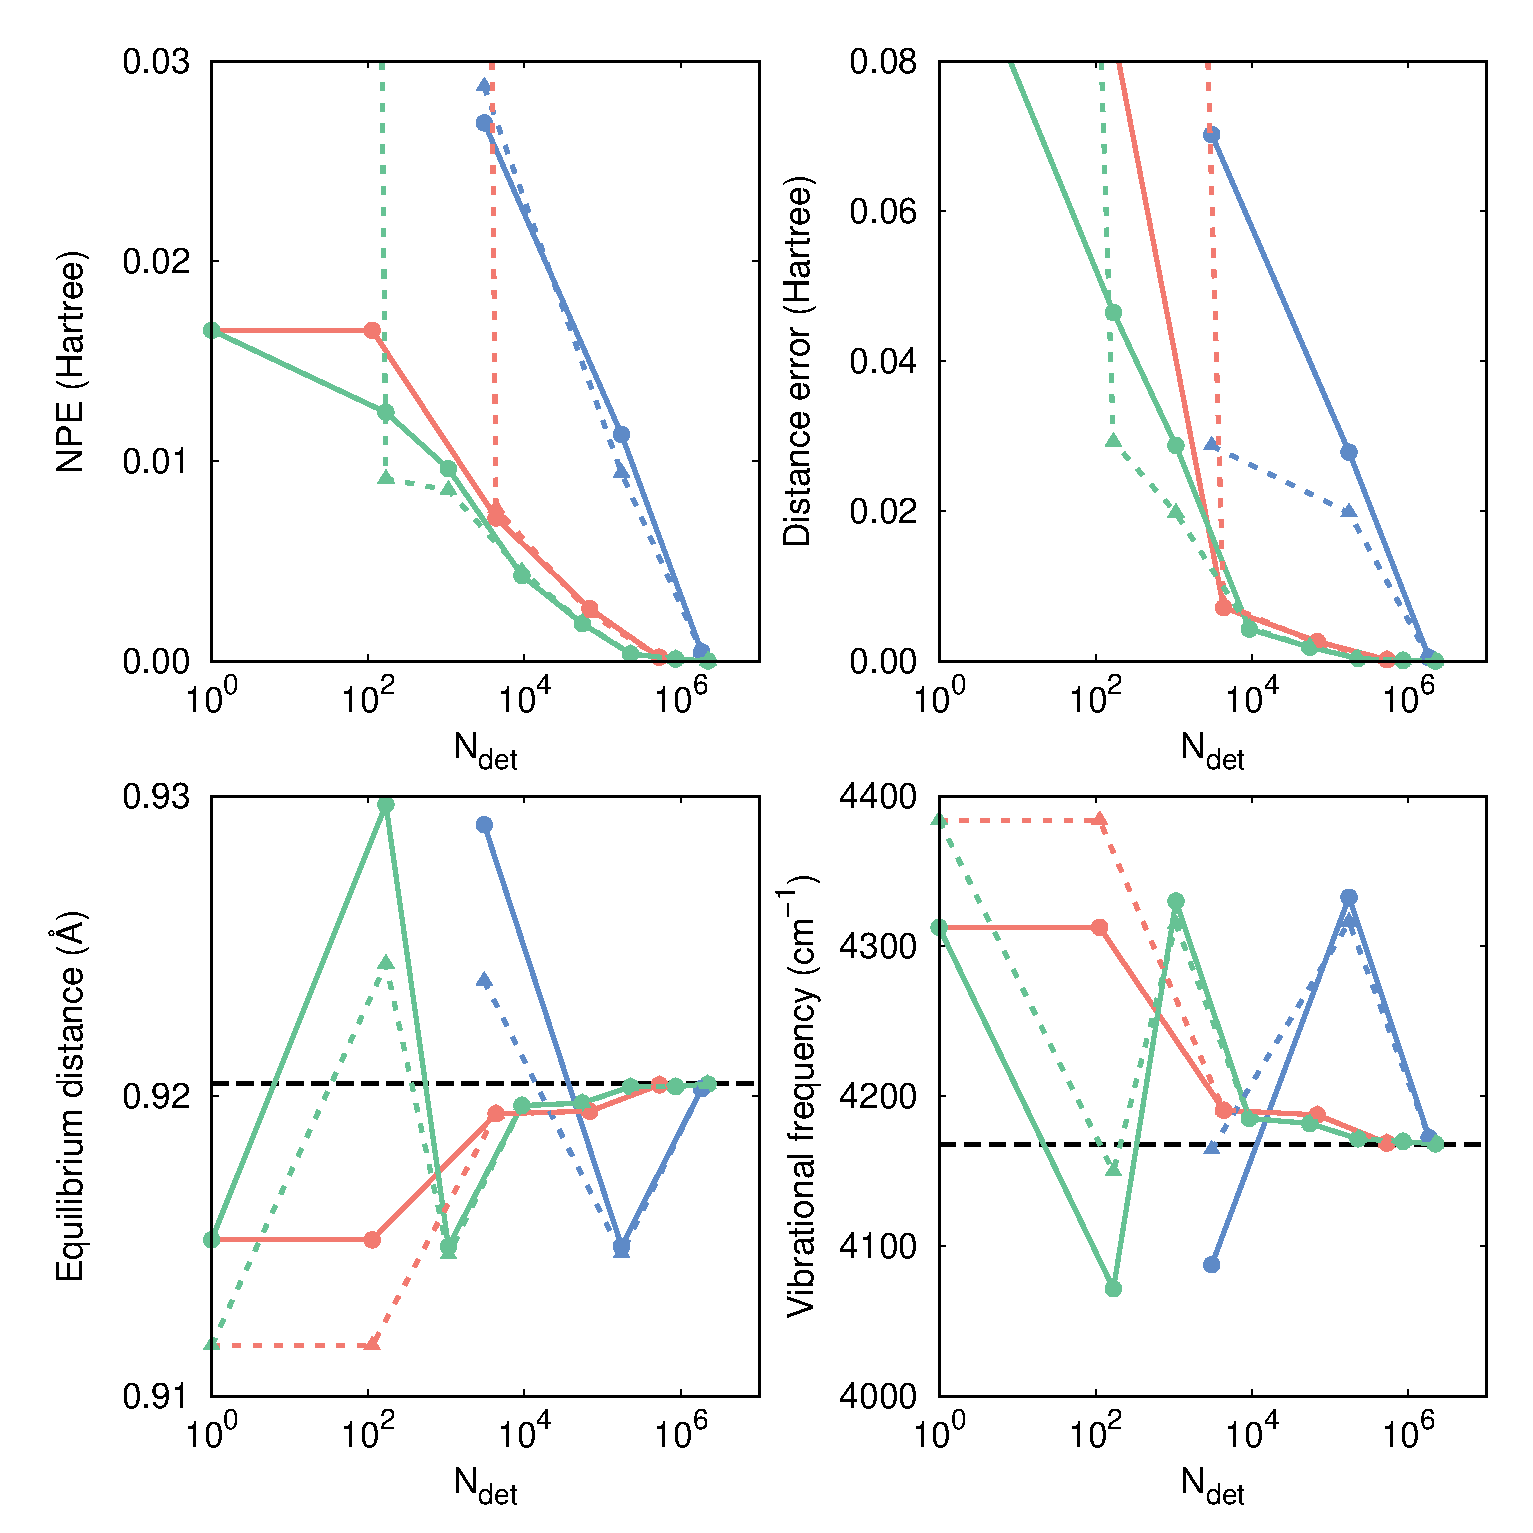
\includegraphics[width=1.0\linewidth]{plot_pt2_rpt2_HF}
\caption{
Non-parallelity error (NPE), distance error, equilibrium distance, and vibrational frequency, for \ce{HF},
as functions of the number of determinants ($\Ndet$), according to hCI (green), eCI (red) and sCI (blue) models,
with the standard (full lines with circles) and renormalized (dashed lines with triangles) EN2 perturbative correction.
The dashed lines represent the FCI results.}
\label{fig:plot_pt2_rpt2_hf}
\end{figure*}
%%% %%% %%%

%%% FIG S7 %%%
\begin{figure*}%[h!]
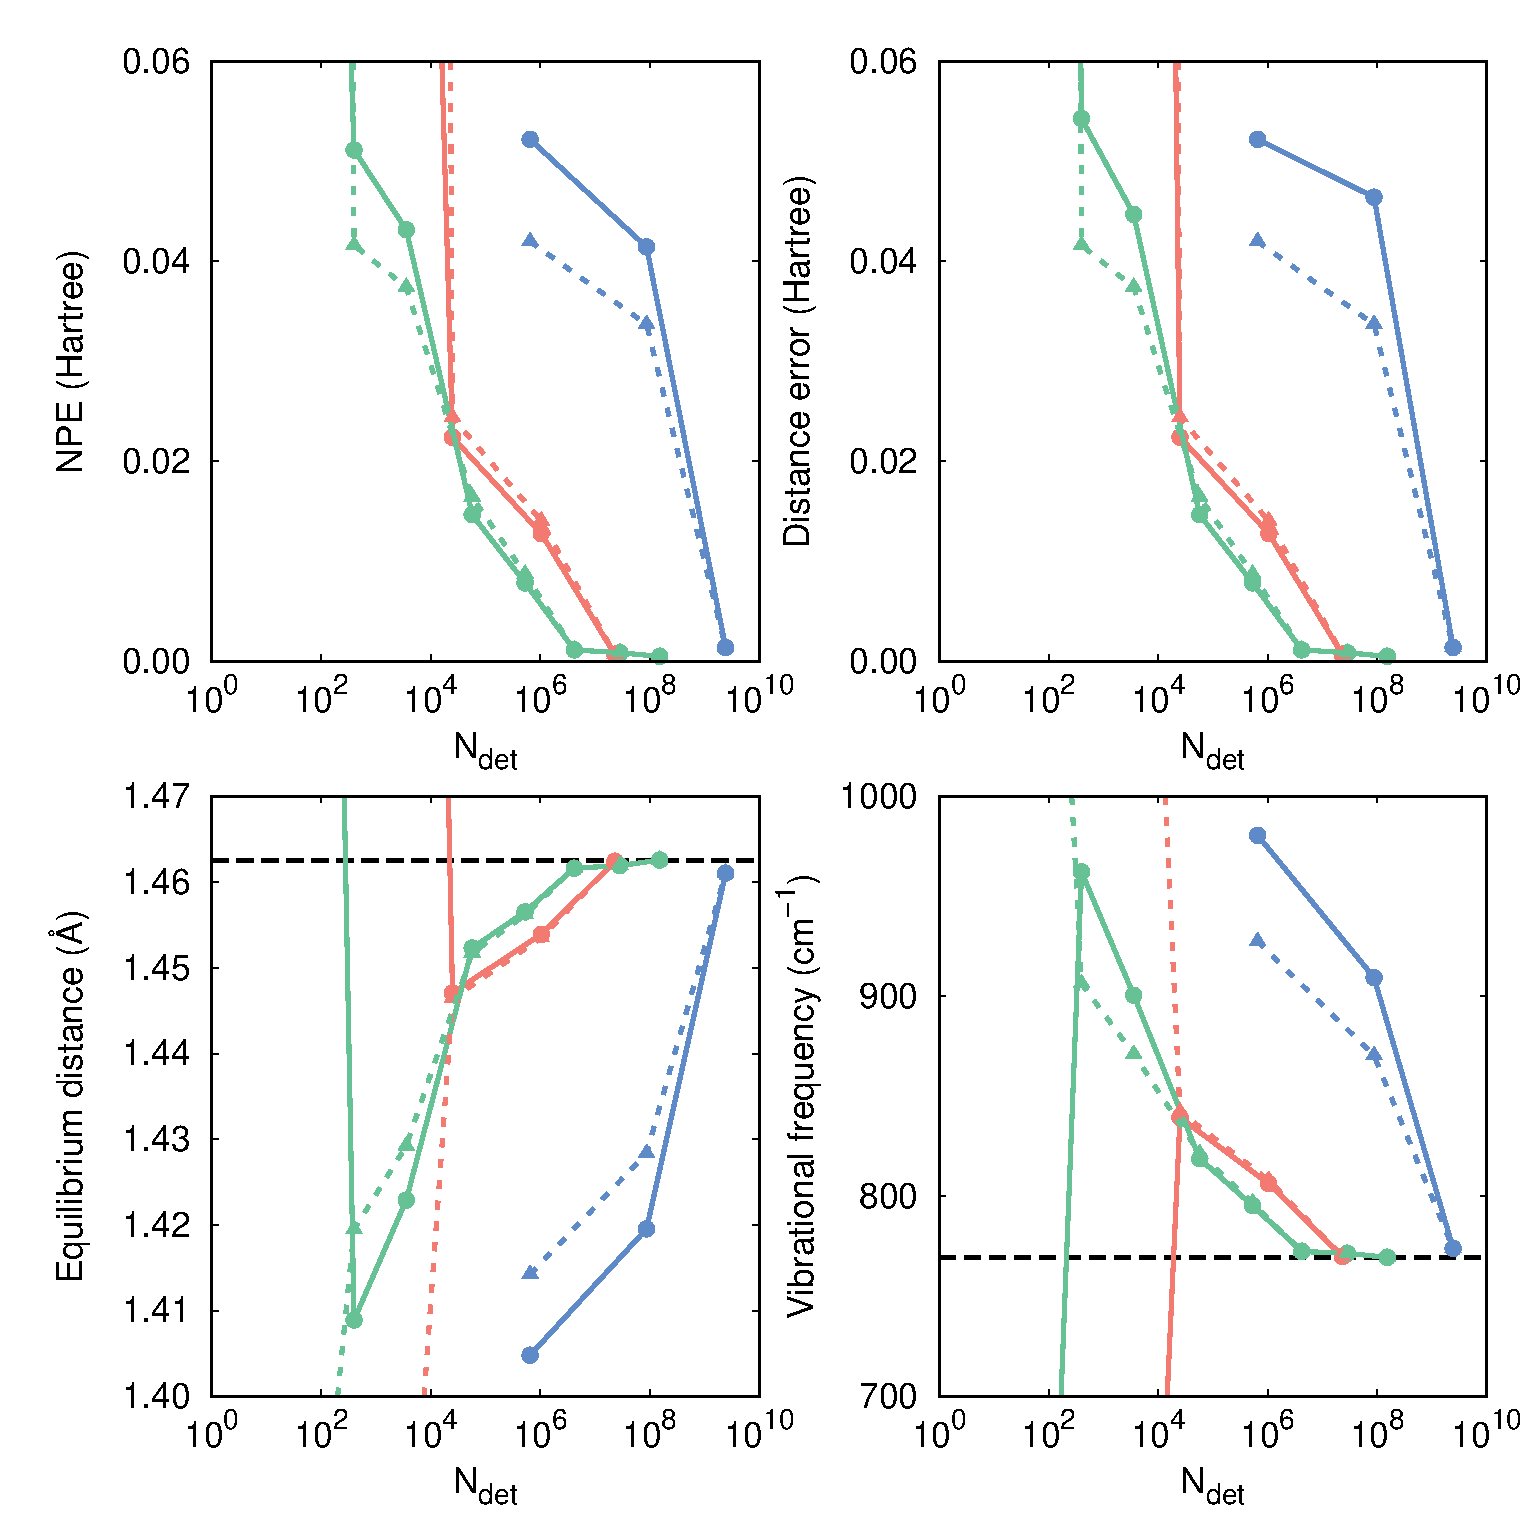
\includegraphics[width=1.0\linewidth]{plot_pt2_rpt2_F2}
\caption{
Non-parallelity error (NPE), distance error, equilibrium distance, and vibrational frequency, for \ce{F2},
as functions of the number of determinants ($\Ndet$), according to hCI (green), eCI (red) and sCI (blue) models,
with the standard (full lines with circles) and renormalized (dashed lines with triangles) EN2 perturbative correction.
The dashed lines represent the FCI results.}
\label{fig:plot_pt2_rpt2_f2}
\end{figure*}
%%% %%% %%%

%%% FIG S8 %%%
\begin{figure*}%[h!]
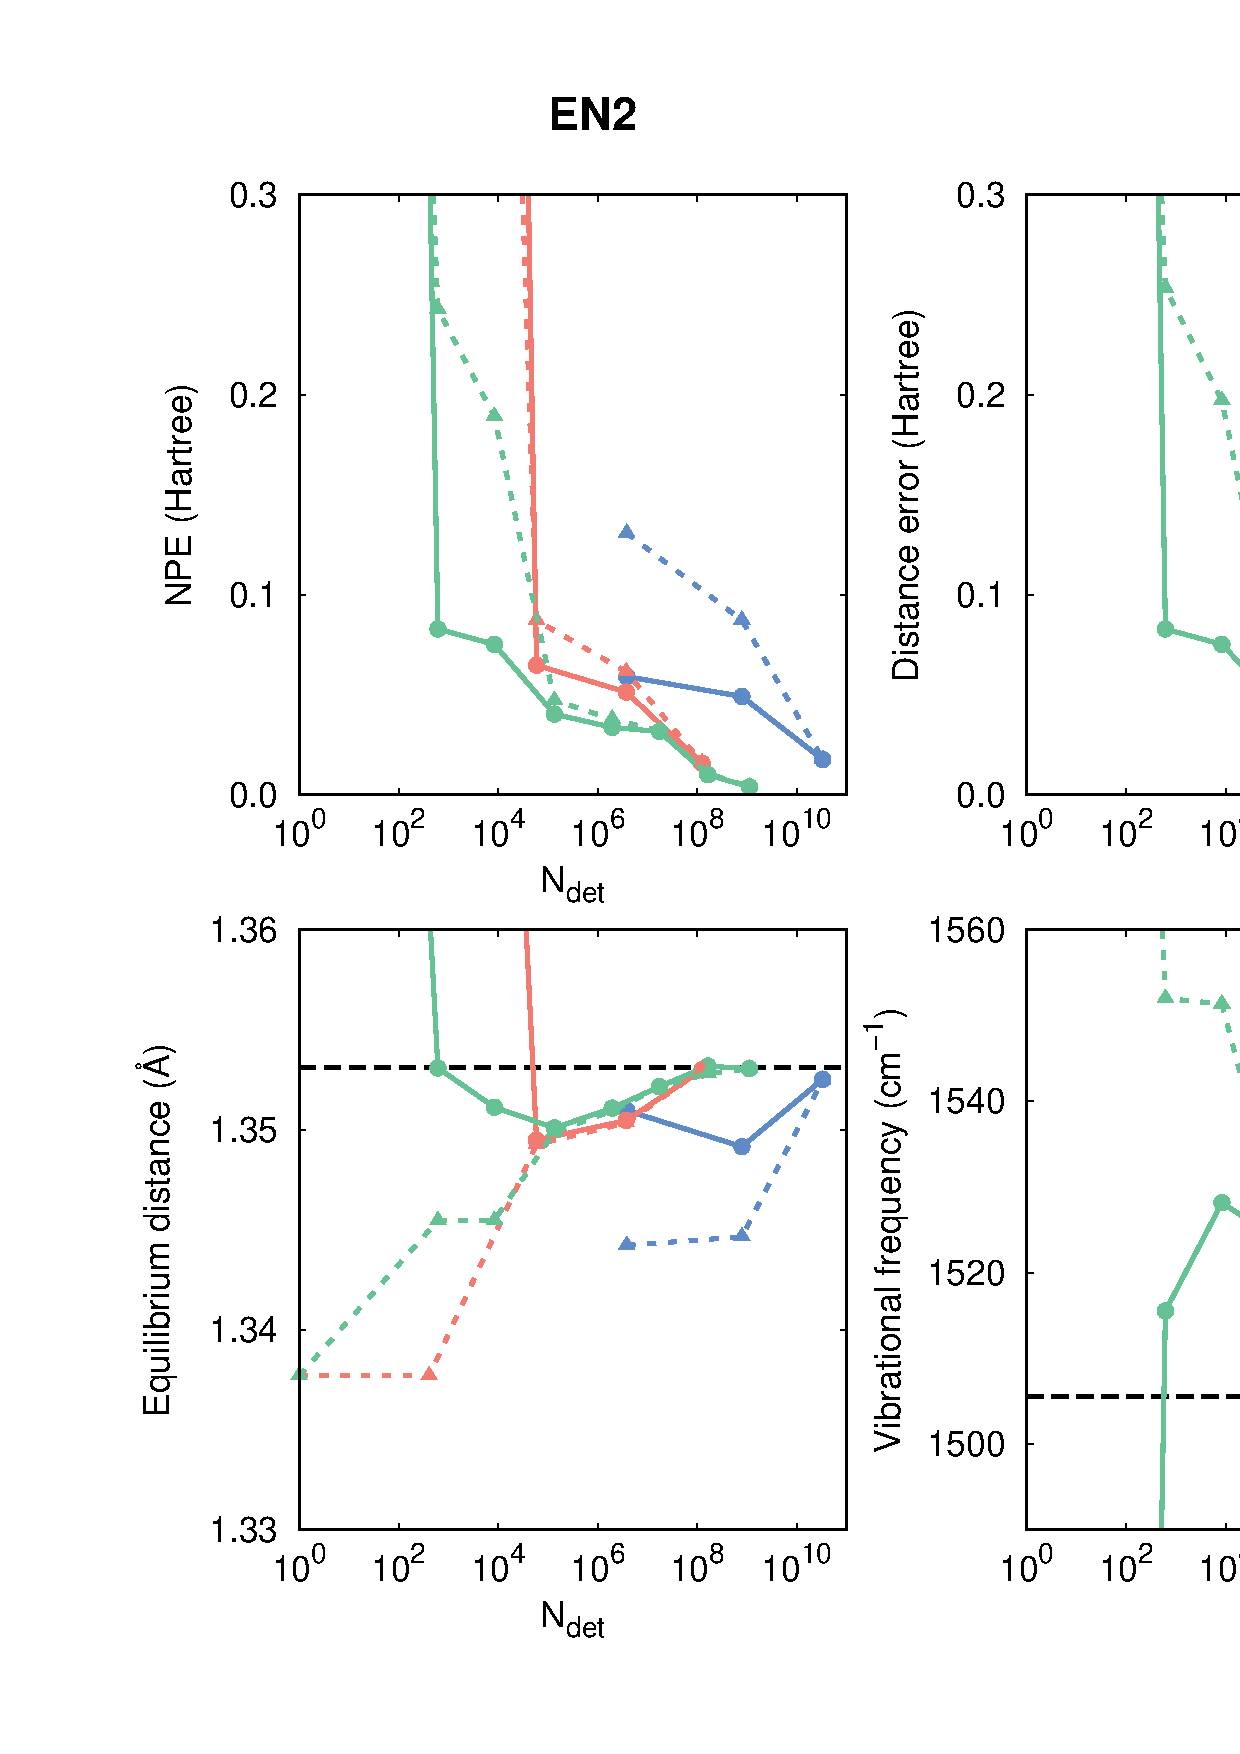
\includegraphics[width=1.0\linewidth]{plot_pt2_rpt2_ethylene}
\caption{
Non-parallelity error (NPE), distance error, equilibrium distance, and vibrational frequency, for ethylene,
as functions of the number of determinants ($\Ndet$), according to hCI (green), eCI (red) and sCI (blue) models,
with the standard (full lines with circles) and renormalized (dashed lines with triangles) EN2 perturbative correction.
The dashed lines represent the FCI results.}
\label{fig:plot_pt2_rpt2_ethylene}
\end{figure*}
%%% %%% %%%

%%% FIG S9 %%%
\begin{figure*}%[h!]
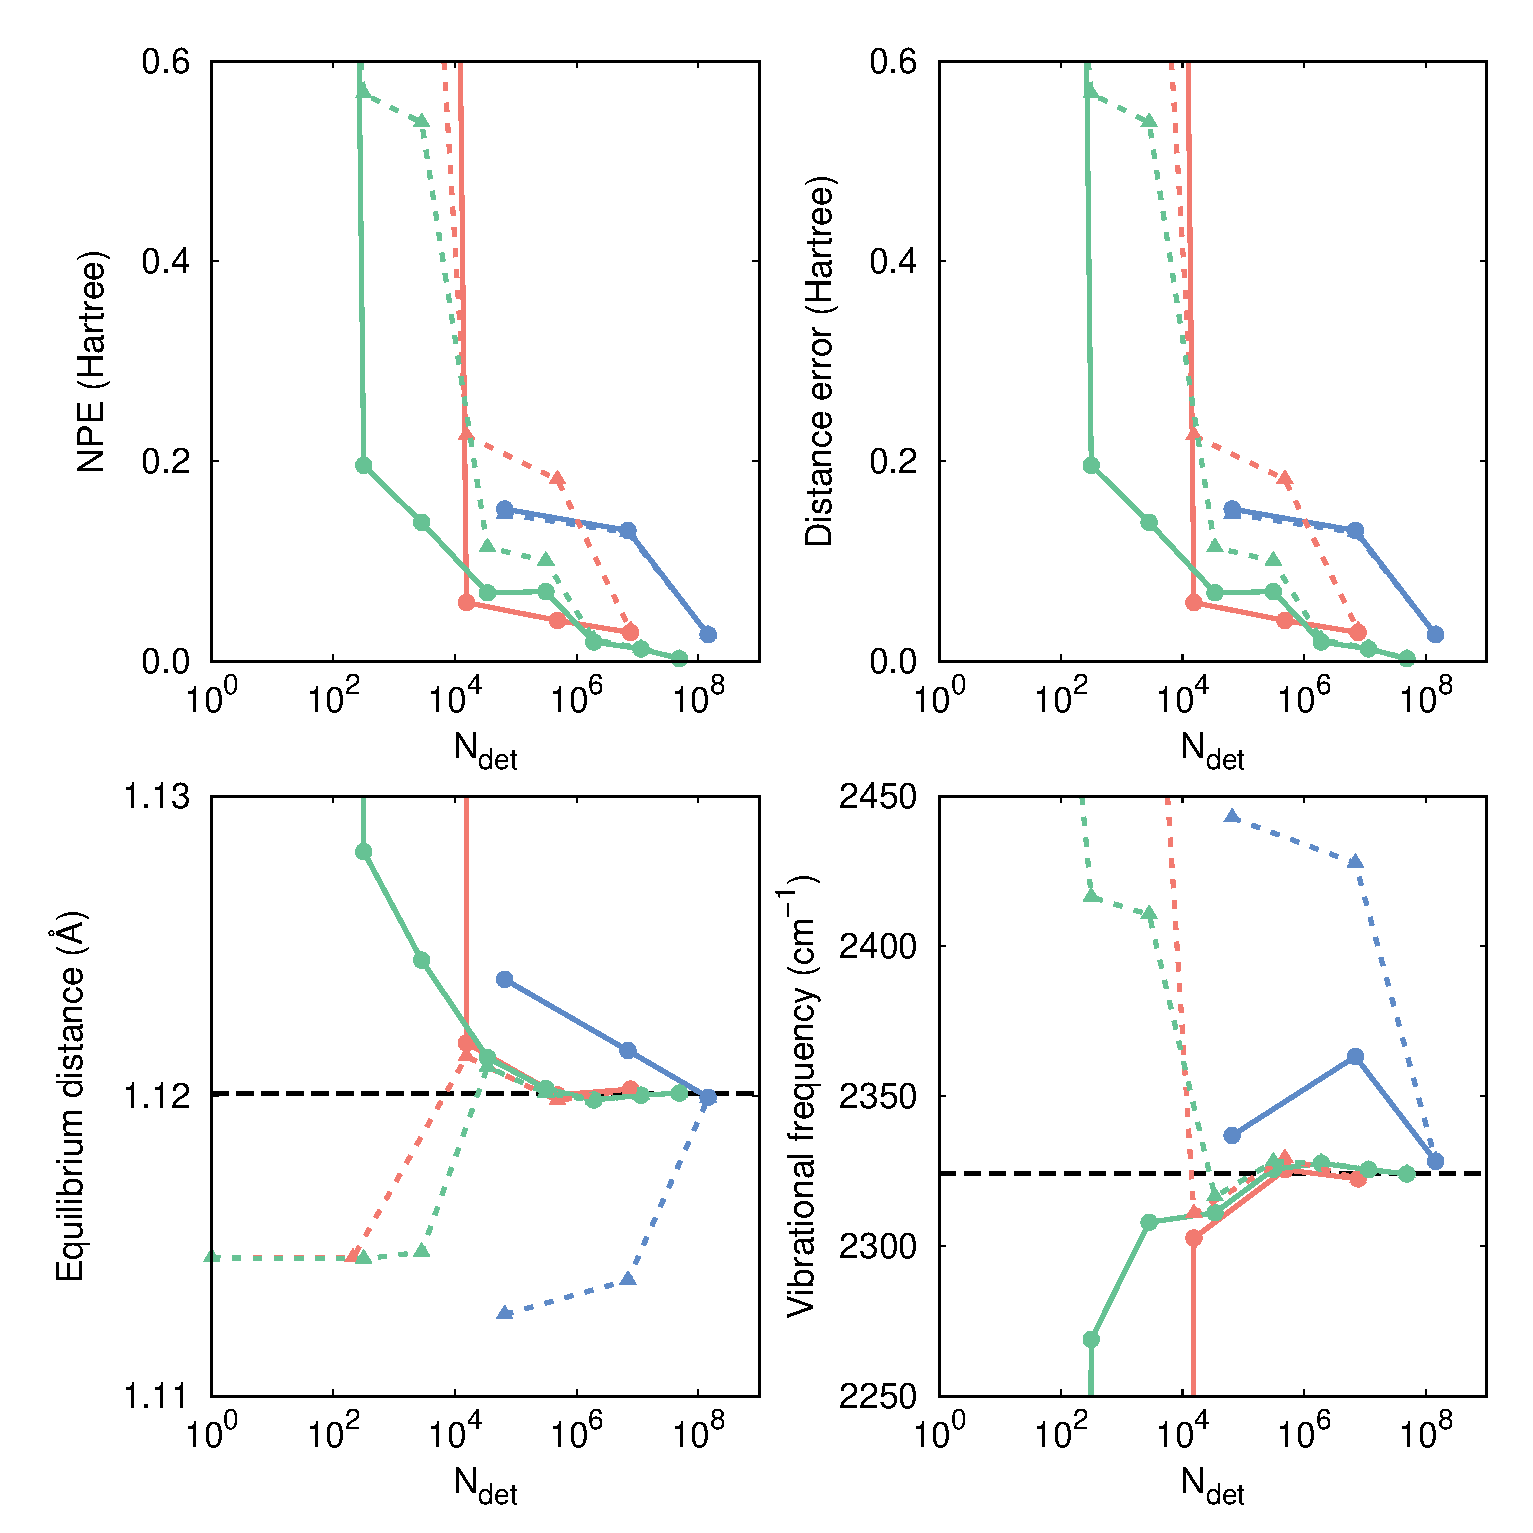
\includegraphics[width=1.0\linewidth]{plot_pt2_rpt2_N2}
\caption{
Non-parallelity error (NPE), distance error, equilibrium distance, and vibrational frequency, for \ce{N2},
as functions of the number of determinants ($\Ndet$), according to hCI (green), eCI (red) and sCI (blue) models,
with the standard (full lines with circles) and renormalized (dashed lines with triangles) EN2 perturbative correction.
The dashed lines represent the FCI results.}
\label{fig:plot_pt2_rpt2_n2}
\end{figure*}
%%% %%% %%%

%%% FIG S10 %%%
\begin{figure*}%[h!]
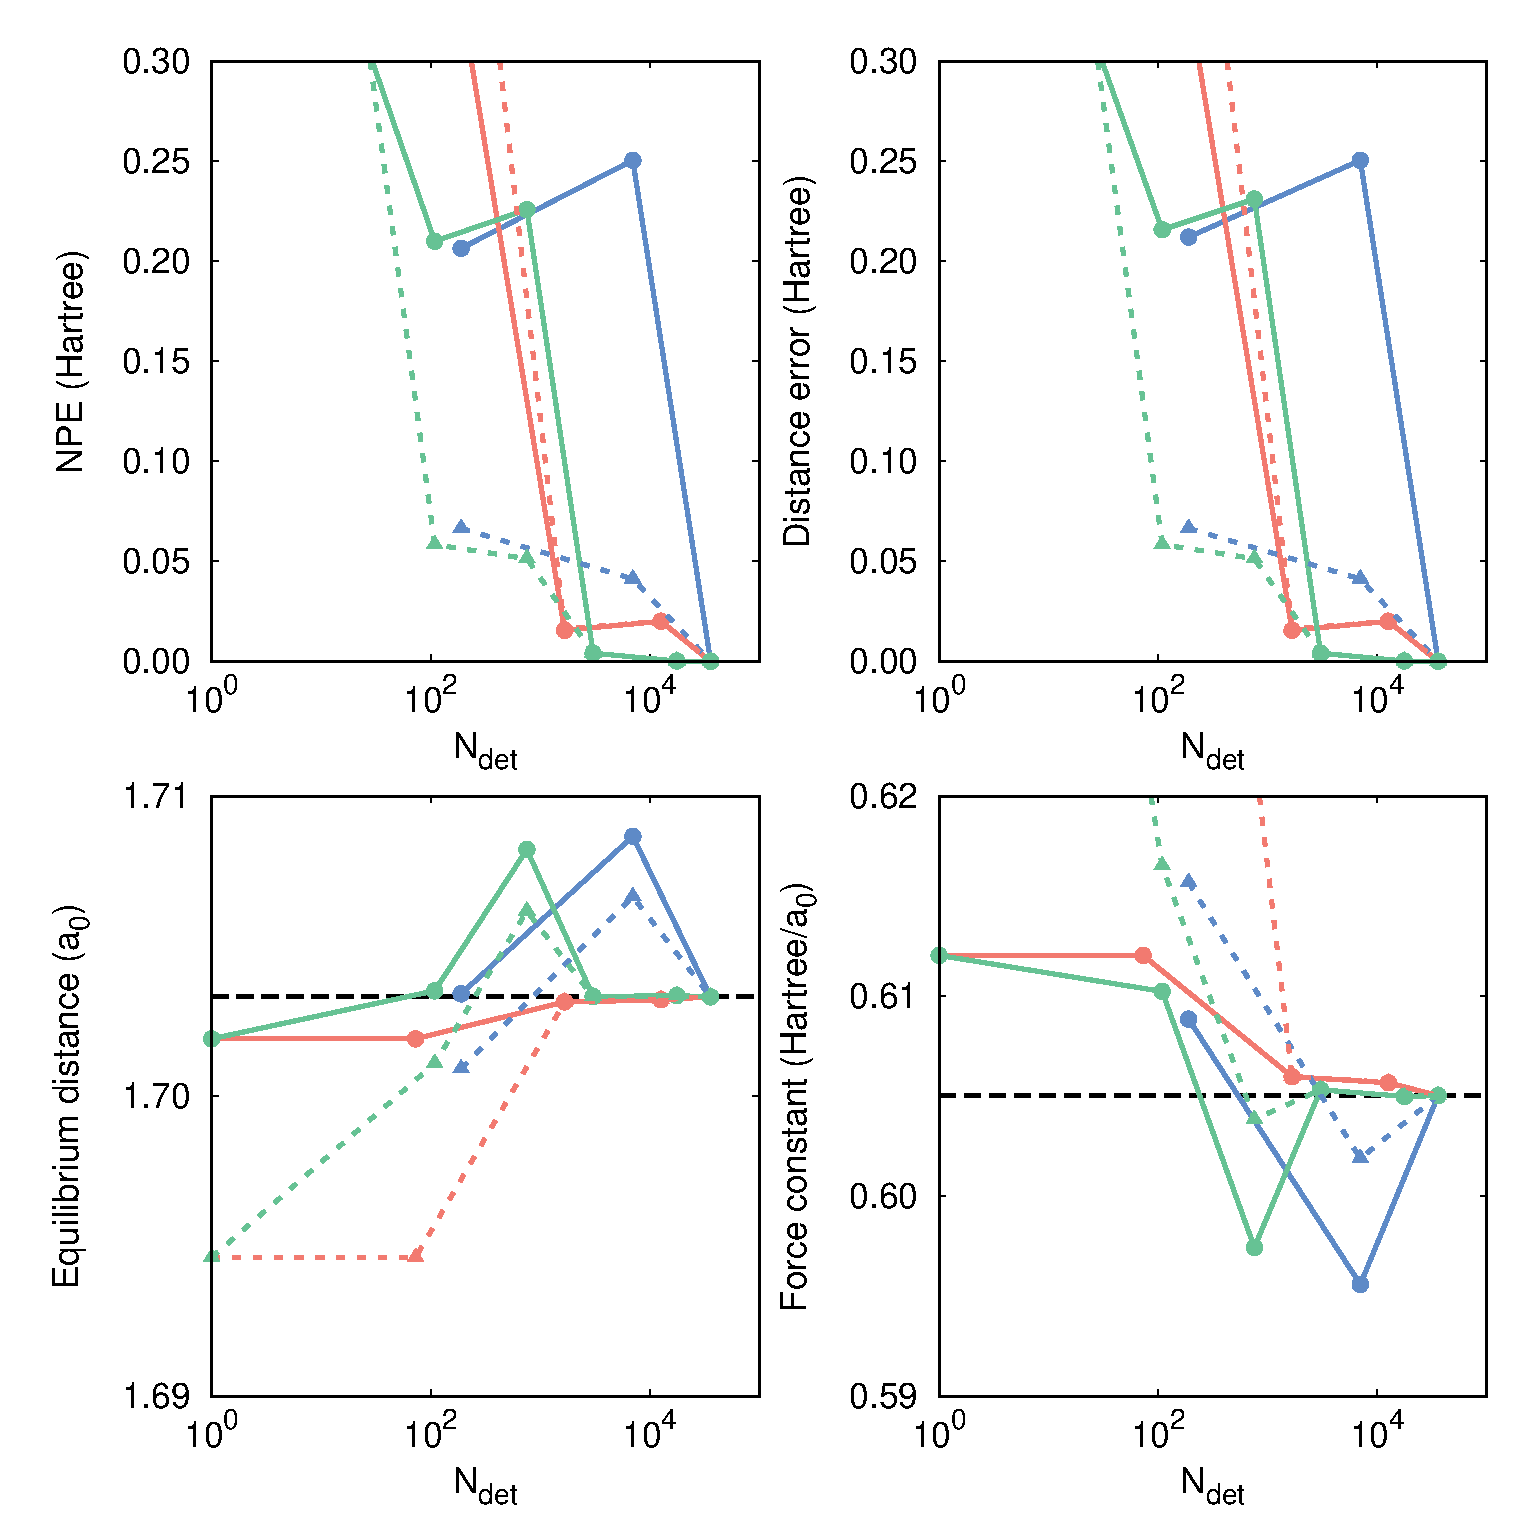
\includegraphics[width=1.0\linewidth]{plot_pt2_rpt2_H4}
\caption{
Non-parallelity error (NPE), distance error, equilibrium distance, and force constant, for \ce{H4},
as functions of the number of determinants ($\Ndet$), according to hCI (green), eCI (red) and sCI (blue) models,
with the standard (full lines with circles) and renormalized (dashed lines with triangles) EN2 perturbative correction.
The dashed lines represent the FCI results.}
\label{fig:plot_pt2_rpt2_h4}
\end{figure*}
%%% %%% %%%

%%% FIG S11 %%%
\begin{figure*}%[h!]
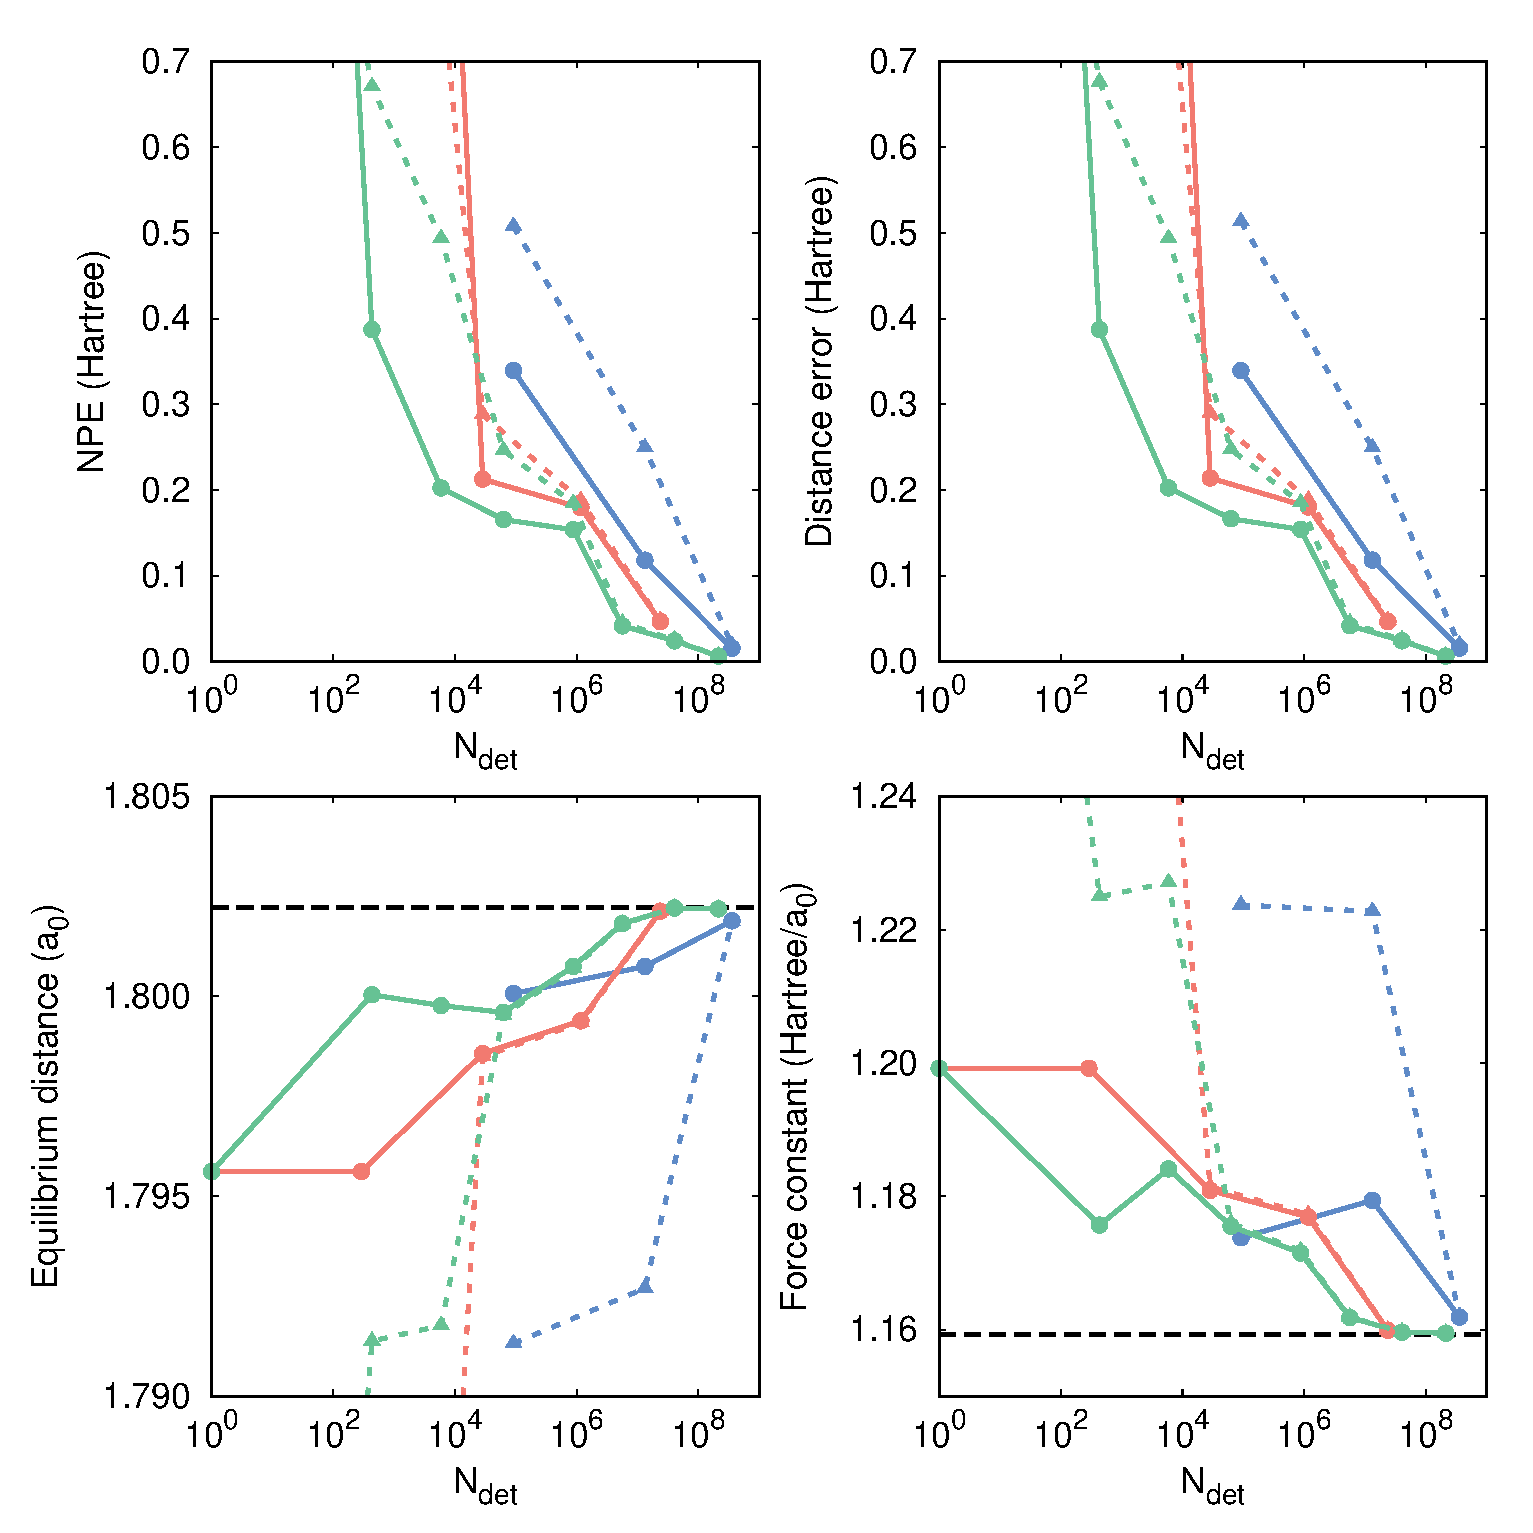
\includegraphics[width=1.0\linewidth]{plot_pt2_rpt2_H8}
\caption{
Non-parallelity error (NPE), distance error, equilibrium distance, and force constant, for \ce{H8},
as functions of the number of determinants ($\Ndet$), according to hCI (green), eCI (red) and sCI (blue) models,
with the standard (full lines with circles) and renormalized (dashed lines with triangles) EN2 perturbative correction.
The dashed lines represent the FCI results.}
\label{fig:plot_pt2_rpt2_h8}
\end{figure*}
%%% %%% %%%

\clearpage

%%%%%%%%%%%%%%%%%%%%%%%%%%%%%%%%
\bibliography{manuscript}
%%%%%%%%%%%%%%%%%%%%%%%%%%%%%%%%

\end{document}
